\documentclass{article}
\usepackage{authblk}
\usepackage{acro}
\usepackage{amsmath}
\usepackage{amsfonts}
\usepackage{caption}
\usepackage{ccaption}
\usepackage[margin=20truemm]{geometry}
\usepackage[dvipdfmx]{graphicx}
\usepackage{hyperref}
\usepackage{url}

\title{
  A graph-based practice of evaluating collective identities of cell clusters
}
\author[1,2]{Yuji Okano}
\author[2,3]{Yoshitaka Kase}
\author[2,3]{Hideyuki Okano}
\affil[1]{
  Department of Extended Intelligence for Medicine, 
  The Ishii-Ishibashi Laboratory, 
  Keio University School of Medicine,
  35 Shinanomachi, Shinjuku-Ku, Tokyo 160-8582, Japan
}
\affil[2]{
  Division of CNS Regeneration and Drug Discovery,
  International Center for Brain Science, 
  Fujita Health University, 
  1-98 Dengakugakubo, Kutsukake-Cho, Toyoake, Aichi 470-1192, Japan
}
\affil[3]{
  Keio University Regenerative Medicine Research Center, 
  3-25-10 Tonomachi, Kawasaki-Ku, Kawasaki, Kanagawa 210-0821, Japan
}
\date{\today}

\DeclareAcronym{scRNA-seq}{short = scRNA-seq, long  = single-cell RNA-sequencing}
\DeclareAcronym{GRN}{short = GRN, long  = gene regulatory network}
\DeclareAcronym{JIM}{short = JIM, long  = Jaccard index matrix}
\DeclareAcronym{DEA}{short = DEA, long  = differential expression analysis}
\DeclareAcronym{DEG}{short = DEG, long  = differentially expressed gene}
\DeclareAcronym{PC}{short = PC, long  = Peter and Clark}
\DeclareAcronym{RPM}{short = RPM, long  = reads per million}
\DeclareAcronym{HVG}{short = HVG, long  = highly variable gene}
\DeclareAcronym{PCA}{short = PCA, long  = principal component analysis}
\DeclareAcronym{TSVD}{short = TSVD, long  = truncated singular value decomposition}
\DeclareAcronym{UMAP}{short = UMAP, long  = uniform manifold approximation and projection}
\DeclareAcronym{ML}{short = ML, long  = machine learning}
\DeclareAcronym{GBDT}{short = GBDT, long  = gradient boosting decision tree}
\DeclareAcronym{GO}{short = GO, long  = gene ontology}
\DeclareAcronym{QC}{short = QC, long  = quality control}
\DeclareAcronym{MMHC}{short = MMHC, long  = max-min hill-climbing}
\DeclareAcronym{OvR}{short = OvR, long  = one-versus-rest}
\DeclareAcronym{AUC}{short = AUC, long  = area under the curve}
\DeclareAcronym{ROC}{short = ROC, long  = receiver operating characteristic}
\DeclareAcronym{AP}{short = AP, long  = average precision}
\DeclareAcronym{PR}{short = PR, long  = precision-recall}
\DeclareAcronym{SHAP}{short = SHAP, long  = Shapley additive explanations}
\DeclareAcronym{DOR}{short = DOR, long  = dropout rate}
\DeclareAcronym{LM}{short = LM, long  = logistic model}
\DeclareAcronym{NB}{short = NB, long  = negative binomial}
\DeclareAcronym{MSE}{short = MSE, long  = mean squared error}
\DeclareAcronym{MAE}{short = MAE, long  = mean absolute error}
\DeclareAcronym{MaxAE}{short = MaxAE, long  = maximum absolute error}
\DeclareAcronym{UMI}{short = UMI, long = unique molecular identifier}
\DeclareAcronym{WHQPM}{short = WHQPM, long = weighted Hamming quasi-pseudo-metric}
\DeclareAcronym{OT}{short = OT, long = optimal transport}


\DeclareCaptionLabelFormat{mainfigs}{\textbf{Figure #2}}
\captionsetup[figure]{labelformat=mainfigs}

\urlstyle{same}

\begin{document}

\maketitle

\section*{Abstract}
The rise of \ac{scRNA-seq} and evolved computational algorithms have significantly advanced 
biomedical science by revealing and visualizing the multifaceted and diverse nature of single cells. These 
technical advancements have also highlighted the pivotal role of cell clusters as representations of biologically universal 
entities such as cell types and cell states. However, to some extent, these clusterings remain dataset-specific and 
method-dependent. To improve comparability across different datasets or compositions, we previously introduced 
a graph-based representation of cell collections that captures the statistical dependencies of their characteristic 
genes.

While our earlier work focused on theoretical insights, it was not sufficiently adapted and fine-tuned for practical 
implementation. To address this, the present paper introduces an improved practice to define and evaluate cellular 
identities based on our theory. First, we provide a concise summary of our previous theory and workflow. Then, 
point-by-point, we highlight the issues that needed fixing and propose solutions. The framework's utility was 
enhanced by leveraging alternative formats of cellular features such as \ac{GO} terms and effectively 
handling dropouts. Supplemental techniques are offered to reinforce the versatility and robustness of our method.

\section*{Introduction}
It has been more than 10 years since the birth of \ac{scRNA-seq} \cite{tang2009mrna}, and the technology is now recognized as a 
prominent game-changer in molecular biology. Like the pioneering technologies in this field---DNA micro array 
and bulk RNA-seq---scRNA-seq can observe multidimensional gene expression profiles. Additionally, it can provide 
such information at the single-cell-level. The abundance of information it provides has contributed to revealing the 
detailed biology of various cell types, but the excessive resolution has blurred the conceptual boundary between static 
cell types and transient cell statuses \cite{regev2017human}. Consequently, ``clusters''---chunks of samples sharing similar geometrical 
properties in the data space---have overwritten the classical notion of cell types. The formation of cell clusters 
depends on the sampling stochasticity of the dataset, and their biological properties might deviate from the original 
doctrine of cell types \cite{okano2023set}. Therefore, a theoretical backbone and an effective method to link theory and experimental 
data are essential to distinguish universal characteristics of specific samples from piles of extrinsic noise.

In our previous research, we proposed a \ac{GRN}-based representation of cell clusters, in 
which the edges of GRNs explain statistical dependencies between two genes. This demonstrated that the similarity 
of two clusters can be defined as a quasi-pseudo-metric function $d^*$ \cite{okano2023set}. To discuss the mathematical properties of 
the quasi-pseudo-metric space of cell clusters, we defined the novel terms ``eigen-cascades'' and ``cell class,'' and 
introduced their algebraic structures. Eigen-cascades refer to a set of marker genes and pairs of genes that are 
statistically interdependent (i.e., isomorphic to the direct sum of the vertex set and the edge set of a GRN). A 
cell class refers to a cell cluster characterized by the corresponding eigen-cascades. Note that the nuances of cell 
cluster and cell class definitions are slightly different, even though we might use those terms interchangeably in this article 
(See Appendices for more explanation). When two cell classes $\forall[x], [y]$ are represented by the GRNs regarding a 
set of genes $G$, and the two GRNs (eigen-cascades) are denoted as $C_{[x]}(G)$ and $C_{[y]}(G)$, a bivariate function $d^*$ 
that maps a pair of cell classes to real numbers is defined as follows \cite{okano2023set}:
\begin{equation}\label{d_asterisk}
  d^*([x], [y]) := 1 - \frac{|C_{[x]}(G)\cap C_{[y]}(G)|}{|C_{[x]}(G)|}.
\end{equation}
Eq. \eqref{d_asterisk} is derived from the Hamming distance function (a metric function that measures the difference between 
two character strings) and modified to embrace the tendency of the \ac{PC} algorithm, one of the 
simplest Bayesian network algorithms \cite{okano2023set,bookstein2002generalized, spirtes2000causation}. With these concepts, we also proposed frameworks to compare 
the similarities of two given cell clusters. Our scheme comprises two fundamental steps: (i) formation of GRNs and (ii) 
evaluation of their similarity (\figurename{ 1A}). As the definition of cell classes is independent of the choice of data 
analysis methods, this framework can be applied into various cases regardless of any feature engineering (such as 
the data preprocessing) or clustering methods.

The framework can be applied into the annotation of scRNA-seq data when a referential dataset is available 
(\figurename{ 1B}). Because annotation is an act of tagging clusters with descriptions in natural languages, the biological 
features of annotated clusters are often treated as common and preserved properties of the cell types after which 
the clusters are named. Accordingly, it is better to have a large enough referential dataset reflecting canonical 
states of specific cell types shared with the query dataset. Using GRN-based characterization, cell classes are annotated 
with the name of the most similar cell class; however, comparisons of cellular identities can be bidirectional due to the 
asymmetry of $d^*$. We refer to the similarity of cell classes from the perspectives of the query data as ``estimation,'' 
and the one from the point of view of the referential data as ``labeling.'' These GRN-based annotations can be 
visualized with planet plots, in which the subjective cell class (denote here as $[x]$) is located in the center and the 
radii of the circles reflect $d^*([x],\cdot)$ values for all cell classes placed on the circumferences.

The performance of those frameworks built around GRNs has a bottleneck in the GRN creation step, which 
involves configuring the vertex sets and choosing of the network algorithm (\figurename{ 1C}). Similar to feature engineering 
and clustering methods, each step of GRN formation offers various options. In our last paper, we introduced a 
combined method of manual curation using review articles and a \ac{ML}-based feature selection 
with a \ac{GBDT} model incorporating L1 and the L2 regularizations \cite{okano2023set}. For manual 
supervision, \ac{GO} terms can serve as an additional information source. However, prior identification of sample 
components is essential to create meaningful GRNs by integrating domain-specific information. The \ac{DEG}-based 
method can be a more heuristic and a less interactive option since the \ac{DEA} 
semi-automatically selects DEGs. Regarding the network algorithms, there are several 
possible options. In our previous paper, we implemented our codes using the numerical (i.e., correlation-based) PC 
algorithms provided in Pgmpy \cite{pgmpy}, a Python package for probabilistic graphical models. Another variation of 
the PC algorithm based on the chi-square test, suitable for categorical data, is also a realistic option when the 
expression values can be binarized. We also mentioned that the \ac{MMHC} algorithm, which 
combines constraint-based and scoring-based methods \cite{tsamardinos2006max}, is one of the promissing alternatives to the PC algorithm.

\begin{figure}[htb]
  \centering
  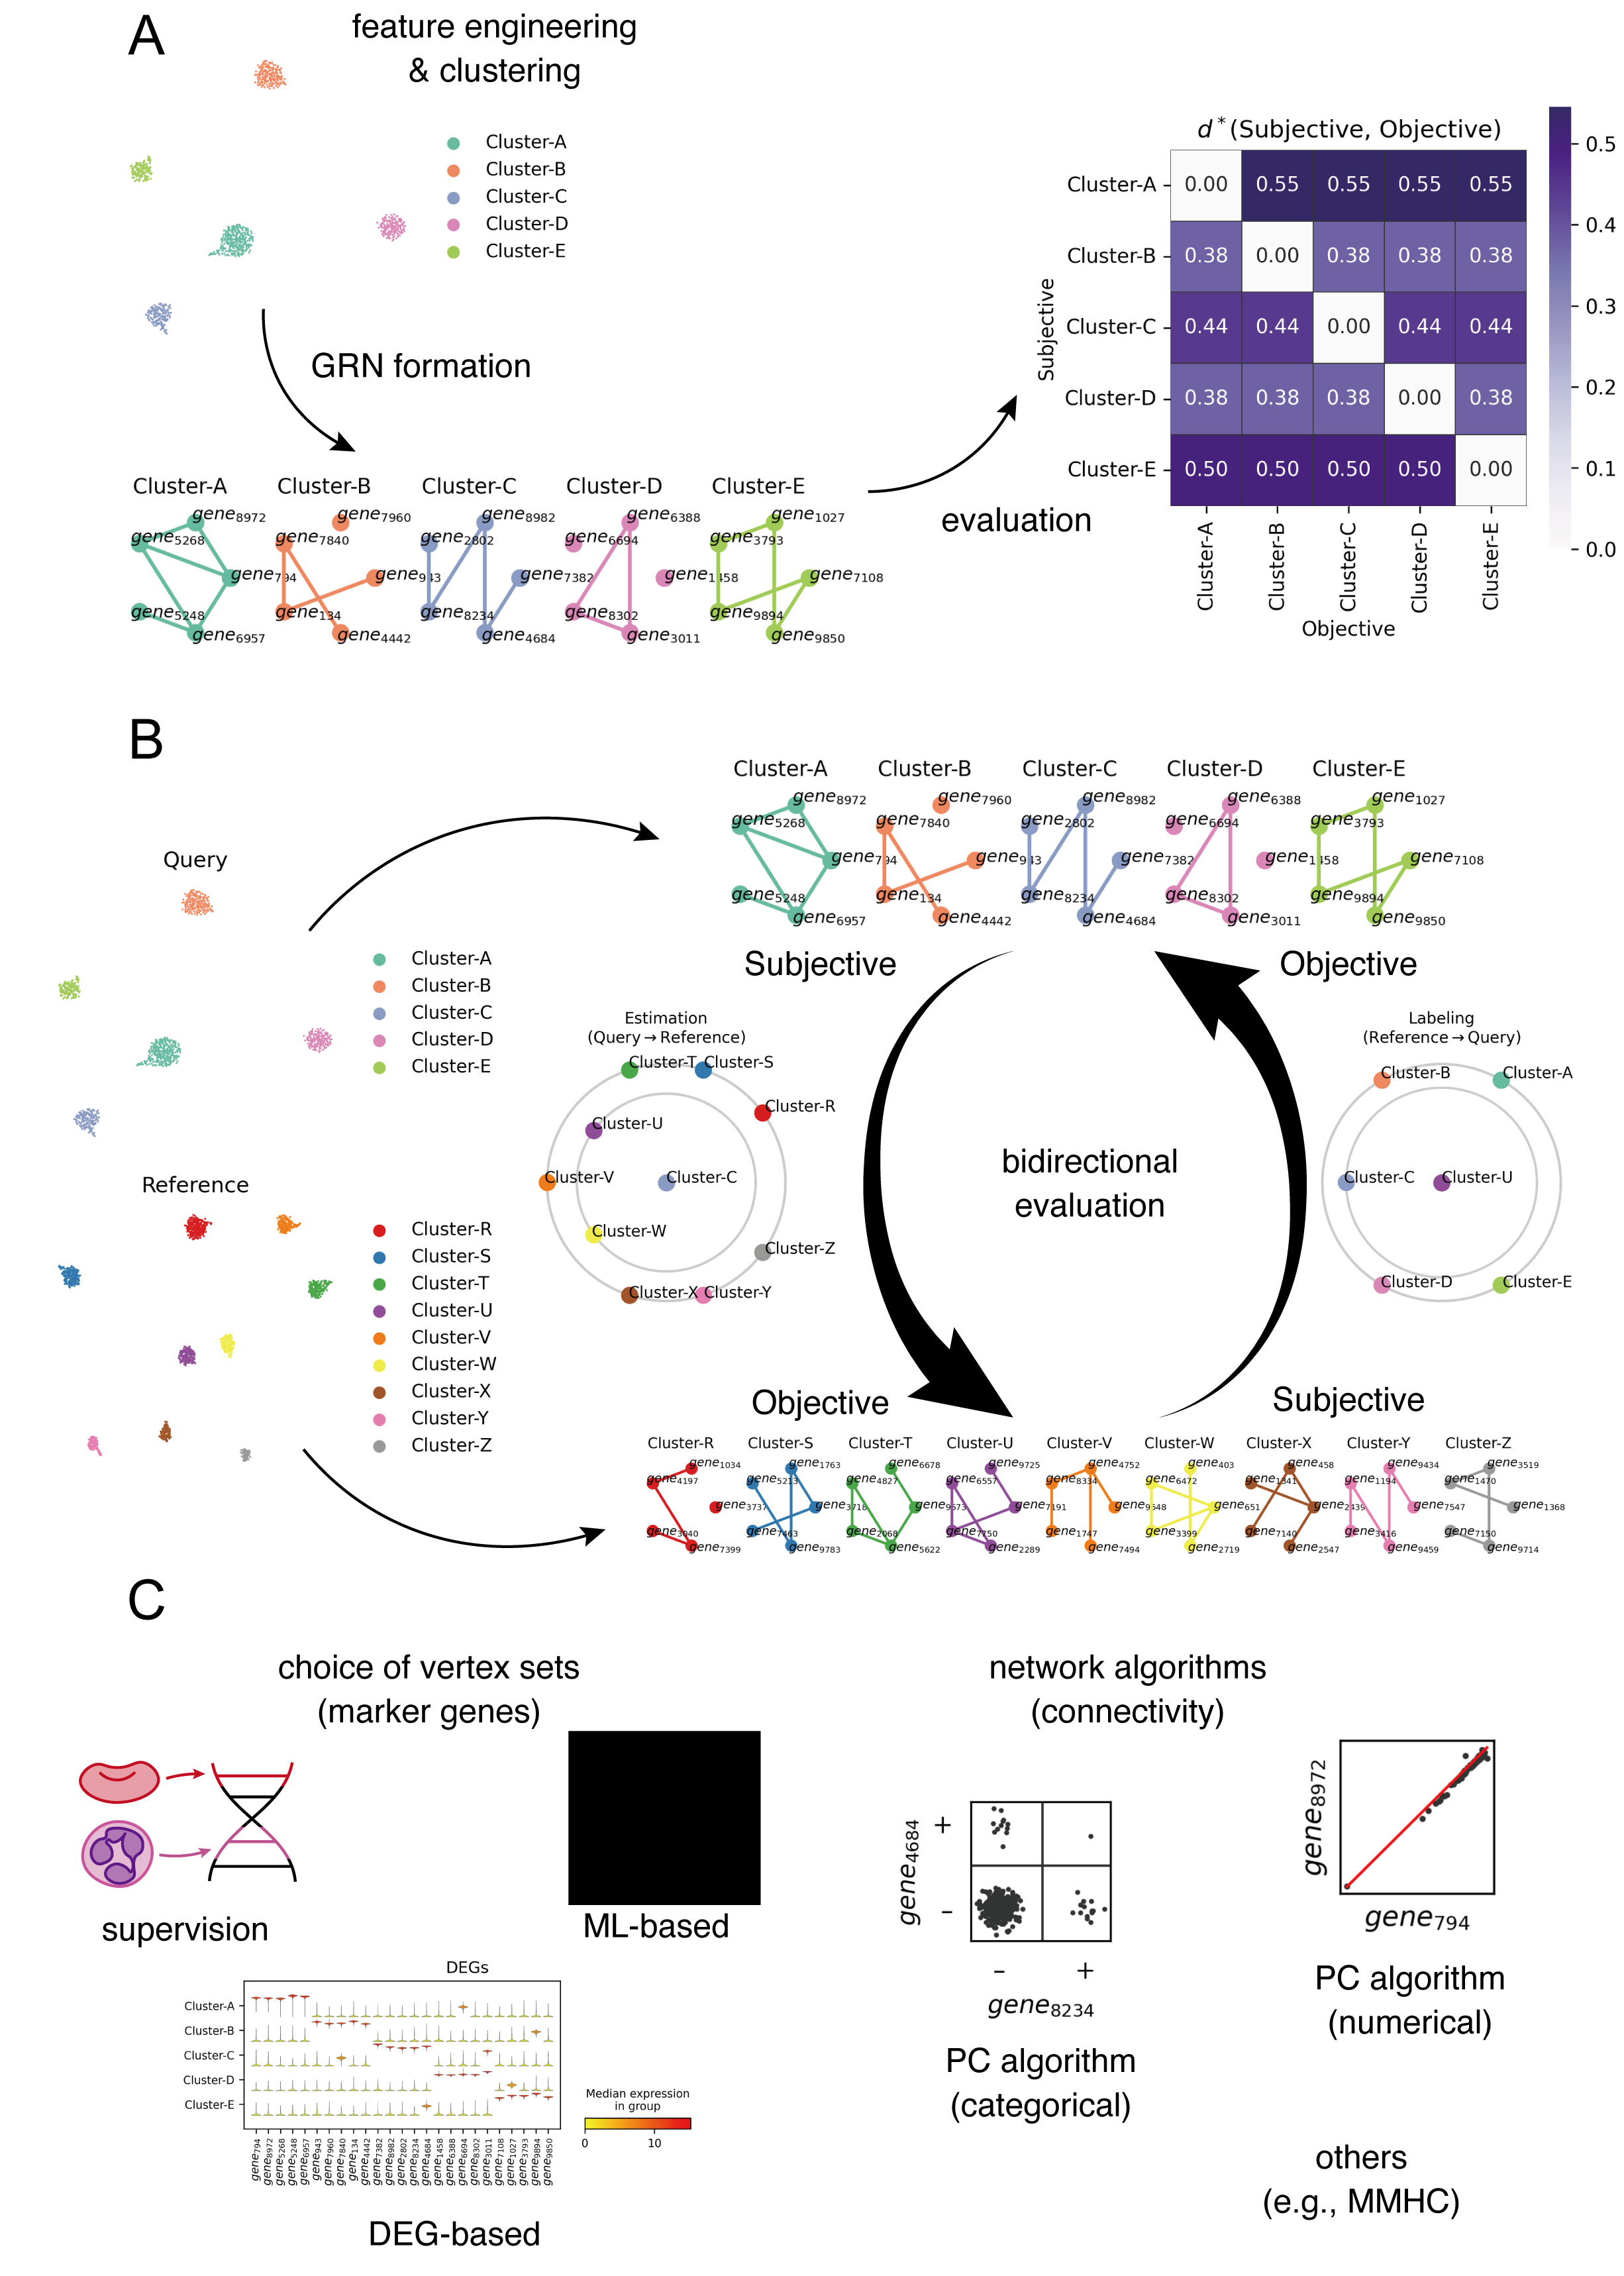
\includegraphics[scale=0.7]{./figs/exported/figure_1.png}
  \caption{The framework of the GRN-based characterization and annotation of cell classes}
  \legend{
    \textbf{A}: The foundation of the GRN-based characterization of cell classes. 
    After clustering in the designated data space by arbitrary methods, cell classes (the clusters) can be represented by 
    GRNs of corresponding genes of choice. The similarity of two GRNs with the same vertex 
    (marker gene) is evaluated with the asymmetrical function $d^*$, where the return values 
    reflect the similarity from the viewpoint of the subjective clusters. 
    \textbf{B}: Schematic of the GRN-based scRNA-seq data annotation. Expecting the referential data to reflect canonical 
    states of target sample domains, the evaluation of the similarity among cell classes can be performed bidirectionally.
    \textbf{C}: Methodological variations of the selection of vertex sets (marker genes) and the algorithms to compute 
    the network structures of GRNs.
  }
  \label{framework}
\end{figure}

So far, we have highlighted the versatility of our framework by providing examples that demonstrate its applicability 
across various data analysis methods. Our intention was to allow researchers to integrate their expertise 
in specific sample domains, or preferences, by textually describing the samples in biological terms. This customization 
ensures that the metrics for cellular identities are crafted to align with the specific research scopes, providing both 
necessary and sufficient resolutions. However, this design choice has the drawback of making our algorithm less 
user-friendly, as it requires a significant amount of effort in annotation, even when annotation might not be a 
primary focus of their projects. To validate our theory across a wide range of cases, it is essential to refine the 
practices related to GRN-based annotation and streamline the overall workflow.

In this article, we address three major issues where the former protocol left room for improvement and provide 
more practical solutions for each while leveraging the backbone theory of GRN-based comparisons of cluster-wise
cellular identities (i.e., cell classes).

\section*{Results}
\subsection*{Challenges for the framework of GRN-based methods}
To clarify our objective for this article, this section describes the three major challenges for the practical use of 
GRN-based annotation:

\subsubsection*{1. Difficulty of effective gene selection}
In our previous study, we proposed a method for selecting marker genes that combines supervised curation, based 
on a review paper, with ML-based feature selection, leveraging the feature importance in an L1-regularized GBDT 
model. While we mentioned that various options exist for marker gene selection, each strategy has its unique 
drawback.

Supervision by the experimenter struggles with completeness and arbitrariness, even when citing reliable sources 
(e.g., review papers or GO terms). For example, in our previous paper, we selected \textit{SLC1A2}, \textit{VIM}, and \textit{AQP4} as 
glial markers based on a review article \cite{zhang2015molecular}. These glial markers are associated with various GO terms, but other 
genes are also tagged with these terms (\figurename{ 2A}). This highlights the incompleteness of these three genes in 
representing all aspects of glia. Furthermore, the many-to-many correspondence between genes and GO terms 
makes it challenging to draw a clear line between adopted marker genes and others.

The ML-based approach is another method we implemented in our last report, and it also has its unique 
problems. As shown in \figurename{ S1}, the standard workflow of scRNA-seq data analysis involves several steps: data \ac{QC}; 
normalization, including \ac{RPM} transformation and logarithmic transformation; 
\ac{HVG} extraction; dimensionality reduction, such as \ac{PCA}, 
\ac{TSVD}, \ac{UMAP} \cite{umap}, 
etc.; clustering; \ac{DEA}; annotation; and other downstream analyses \cite{luecken2019current}. Creating an effective ML model requires 
considerable time beyond actual run times for fine-tuning model configurations, which can be excessively effortful 
for gene selection for GRNs, especially when annotation is not the primary goal of the data analysis. Moreover, even 
with a well-performing ML model, extracting informative features can suffer from arbitrariness in the selection. 
To illustrate these difficulties, we analyzed an open-source scRNA-seq dataset of peripheral blood mononuclear cells 
(referred to as ``PBMC3k'' for convenience), distributed bt the company 10X Genomics. Starting from QC, 
we proceeded to leiden clustering, resulting in 9 clusters (0$\sim$8) as shown in \figurename{ 2B}. We then created a GBDT 
model for multiclass classification, predicting clusters from gene expression values. The model performed well in terms 
of the \ac{AUC} of the \ac{OvR} \ac{ROC} curves; 
the macro average of the OvR ROC curves; the \ac{AP} of the \ac{OvR} \ac{PR} curves; 
the micro average of the OvR PR curves; and the accuracy score (\figurename{ S2A-D}). In our previous article, we created a 
three-class classification model and used feature importance as a criterion (\figurename{ 2C}). However, this approach did 
not work for the nine-class classification model due to the lack of clear boundaries between key and negligible features, 
even when selecting the top 10 features of importance. Since GRNs require pairwise edge calculation, 
modelers should avoid using an excessive number of genes for computational efficiency. Besides feature importance 
scores, \ac{SHAP} scores can be an alternative metric to visualize the correspondence between features 
and classifications \cite{shap}. Despite SHAP scores providing more intuitive and precise explanations 
(\figurename{ 2D and S3A-I}), it remains challenging to introduce objective thresholds for gene selection due to the drastically 
varying distributions of SHAP scores across different classes. Consequently, the ML-based approach is not the most 
effective way to select marker genes for representing cell classes, as it requires subjective and case-by-case decisions on the 
number of marker genes to adopt, making it more time-consuming. ML-based approaches might work well if the 
character of the samples is completely unknown or the consensus among experts is yet to be settled. However, even 
under such conditions, alternative methods such as the DEG-based approach should be considered.

The DEG-based approach is another alternative that can be smoothly integrated into the regular scRNA-seq 
data analysis pipeline. Despite its heuristic nature and promptness, this method also has its shortcomings. Using 
the PBMC3k data processed the same way as in the previous section, we will illustrate this with an example. The 
GRN-based approach offers the advantage of a swift procedure by directly applying the top DEGs into the vertex 
sets. Accordingly, we applied the top 5 DEGs of each cluster to the vertex sets (\figurename{ S4A}), created GRNs based 
on those genes (\figurename{ S4B}), and calculated the $d^*$ values (\figurename{ 2E}). Observing the bottom row of the heatmap, 
the $d^*$ values were all zero from the perspective of cluster 8 even though it showed significantly different expression 
patterns of the top 5 marker genes (\figurename{ 2F}). Additionally, the top 30 upregulated GO terms of each cluster 
indicate that cluster 8 could exclusively be annotated as ``megakaryocytes,'' while the others exhibited different 
cellular characters (\figurename{ S5A-I}). This indicated that the GRNs did not work properly for identifying cluster 8, 
as the zero $d^*$ values for the clusters 0$\sim$7 implied that these clusters and cluster 8 were indistinguishable in terms 
of the GRNs with the given vertex sets. Increasing the number of DEGs to 10 added an edge to the GRN for 
cluster 8, resulting in non-zero $d^*$ values (\figurename{ 2H-I}). As the GO terms suggested no other clusters of megakaryocytes 
except cluster 8, the new $d^*$ values appeared to correctly indicate that the clusters 0$\sim$7 were equally different from 
cluster 8. Thus, the marker-gene selection is an intricate step that requires repetitive adjustments and validations 
especially when exploring the optimal number of the DEGs to use for the vertex sets.

In this paragraph, we have highlighted issues with various marker-gene selection methods and emphasized that 
selecting necessary and sufficient genes to represent certain cellular identities is time-consuming and sometimes 
computationally intensive, though it is a key part of GRN-based annotation. Given this, and considering that 
annotation is often not the ultimate goal of the scRNA-seq data analyses, developing an alternative method for 
finding marker genes is necessary to reduce computational costs and streamline the time required before initiating 
the main analyses.


\subsubsection*{2. Statistical issue: independence v.s. uncorrelation}
The statistical independence of two events $A$ and $B$ is defined as a situation where the following equation holds:
\begin{equation}\label{independence}
  P(A\cap B)=P(A)P(B),
\end{equation}
where $P(\cdot)$ is the probability of an event. On the other hand, the correlation coefficient $Corr(X, Y)$ of stochastic variables 
$X$ and $Y$ is defined as follows:
\begin{equation}\label{corr}
  Corr(X, Y):=\frac{Cov(X, Y)}{\sqrt{Var[X]Var[Y]}},\quad \text{if}\; Var[X]Var[Y] > 0,
\end{equation}
where $E[\cdot]$ is the expected value, $Var[\cdot]$ is the variance, and $Cov(\cdot, \cdot)$ is the covariance. Independent variables exhibit 
a correlation coefficient of zero, but the converse is false. For example, if $X\sim U(-1, 1)$, where $U(-1, 1)$ refers to 
the uniform distribution over the interval from -1 to 1, then $Corr(X, X^2)=0$ although $X$ and $X^2$ are dependent. 
Therefore, strictly speaking, it is not appropriate to substitute the chi-square test or the exact test with the t-test 
of correlation. Furthermore, the correlation-based method does not work well when the gene expression matrices are 
highly sparse regarding the selected genes. As Eq. \eqref{corr} holds if, and only if, both $Var[X]$ and $Var[Y]$ are non-zero 
values, under circumstances where all samples in a cluster exhibit zero counts for certain genes required 
in the vertex set, the correlation-based approach is inappropriate. This situation is by no means an unrealistic 
hypothetical counterexample. For example, a phenomenon called ``dropout'' is a characteristic of scRNA-seq data 
where gene expressions are not detected due to the inefficiency and the stochasticity of scRNA-seq \cite{qiu2020embracing}, resulting 
in high sparsity of scRNA-seq data matrices.

In our previous work, we introduced a correlation-based algorithm to construct GRNs, compromising rigor to 
accommodate continuous gene expression values. To address this issue in the current study, we propose 
an effective method to binarize the gene expression values, allowing the new algorithm to rely on statistical tests of 
independence. This update will better aligh our algorithm with the original concept of our theory.

\subsubsection*{3. Insufficient responsiveness to gene expression values}
GRNs have originally been designed to represent cellular functions by establishing edges between two statistically 
dependent genes. The correlation-based GRN generation follows the same idea, drawing edges between two vertexes 
where correlations exist. Although these strategies can visualize the co-occurrence or mutual exclusivity of the gene 
expressions, actual expression values are dismissed. This failure leads to misassignments of cellular identities in 
practical cases, as demonstrated with the PBMC3k example; namely, the GRNs of clusters 0 and 8 showed identical 
structures despite significantly different expression patterns of the marker genes forming the vertex set (\figurename{ 2F-G}). 
This example highlights not only the difficulty of the gene selection but also the insufficient responsiveness 
of GRNs to gene expression values.

\begin{figure}[htb]
  \centering
  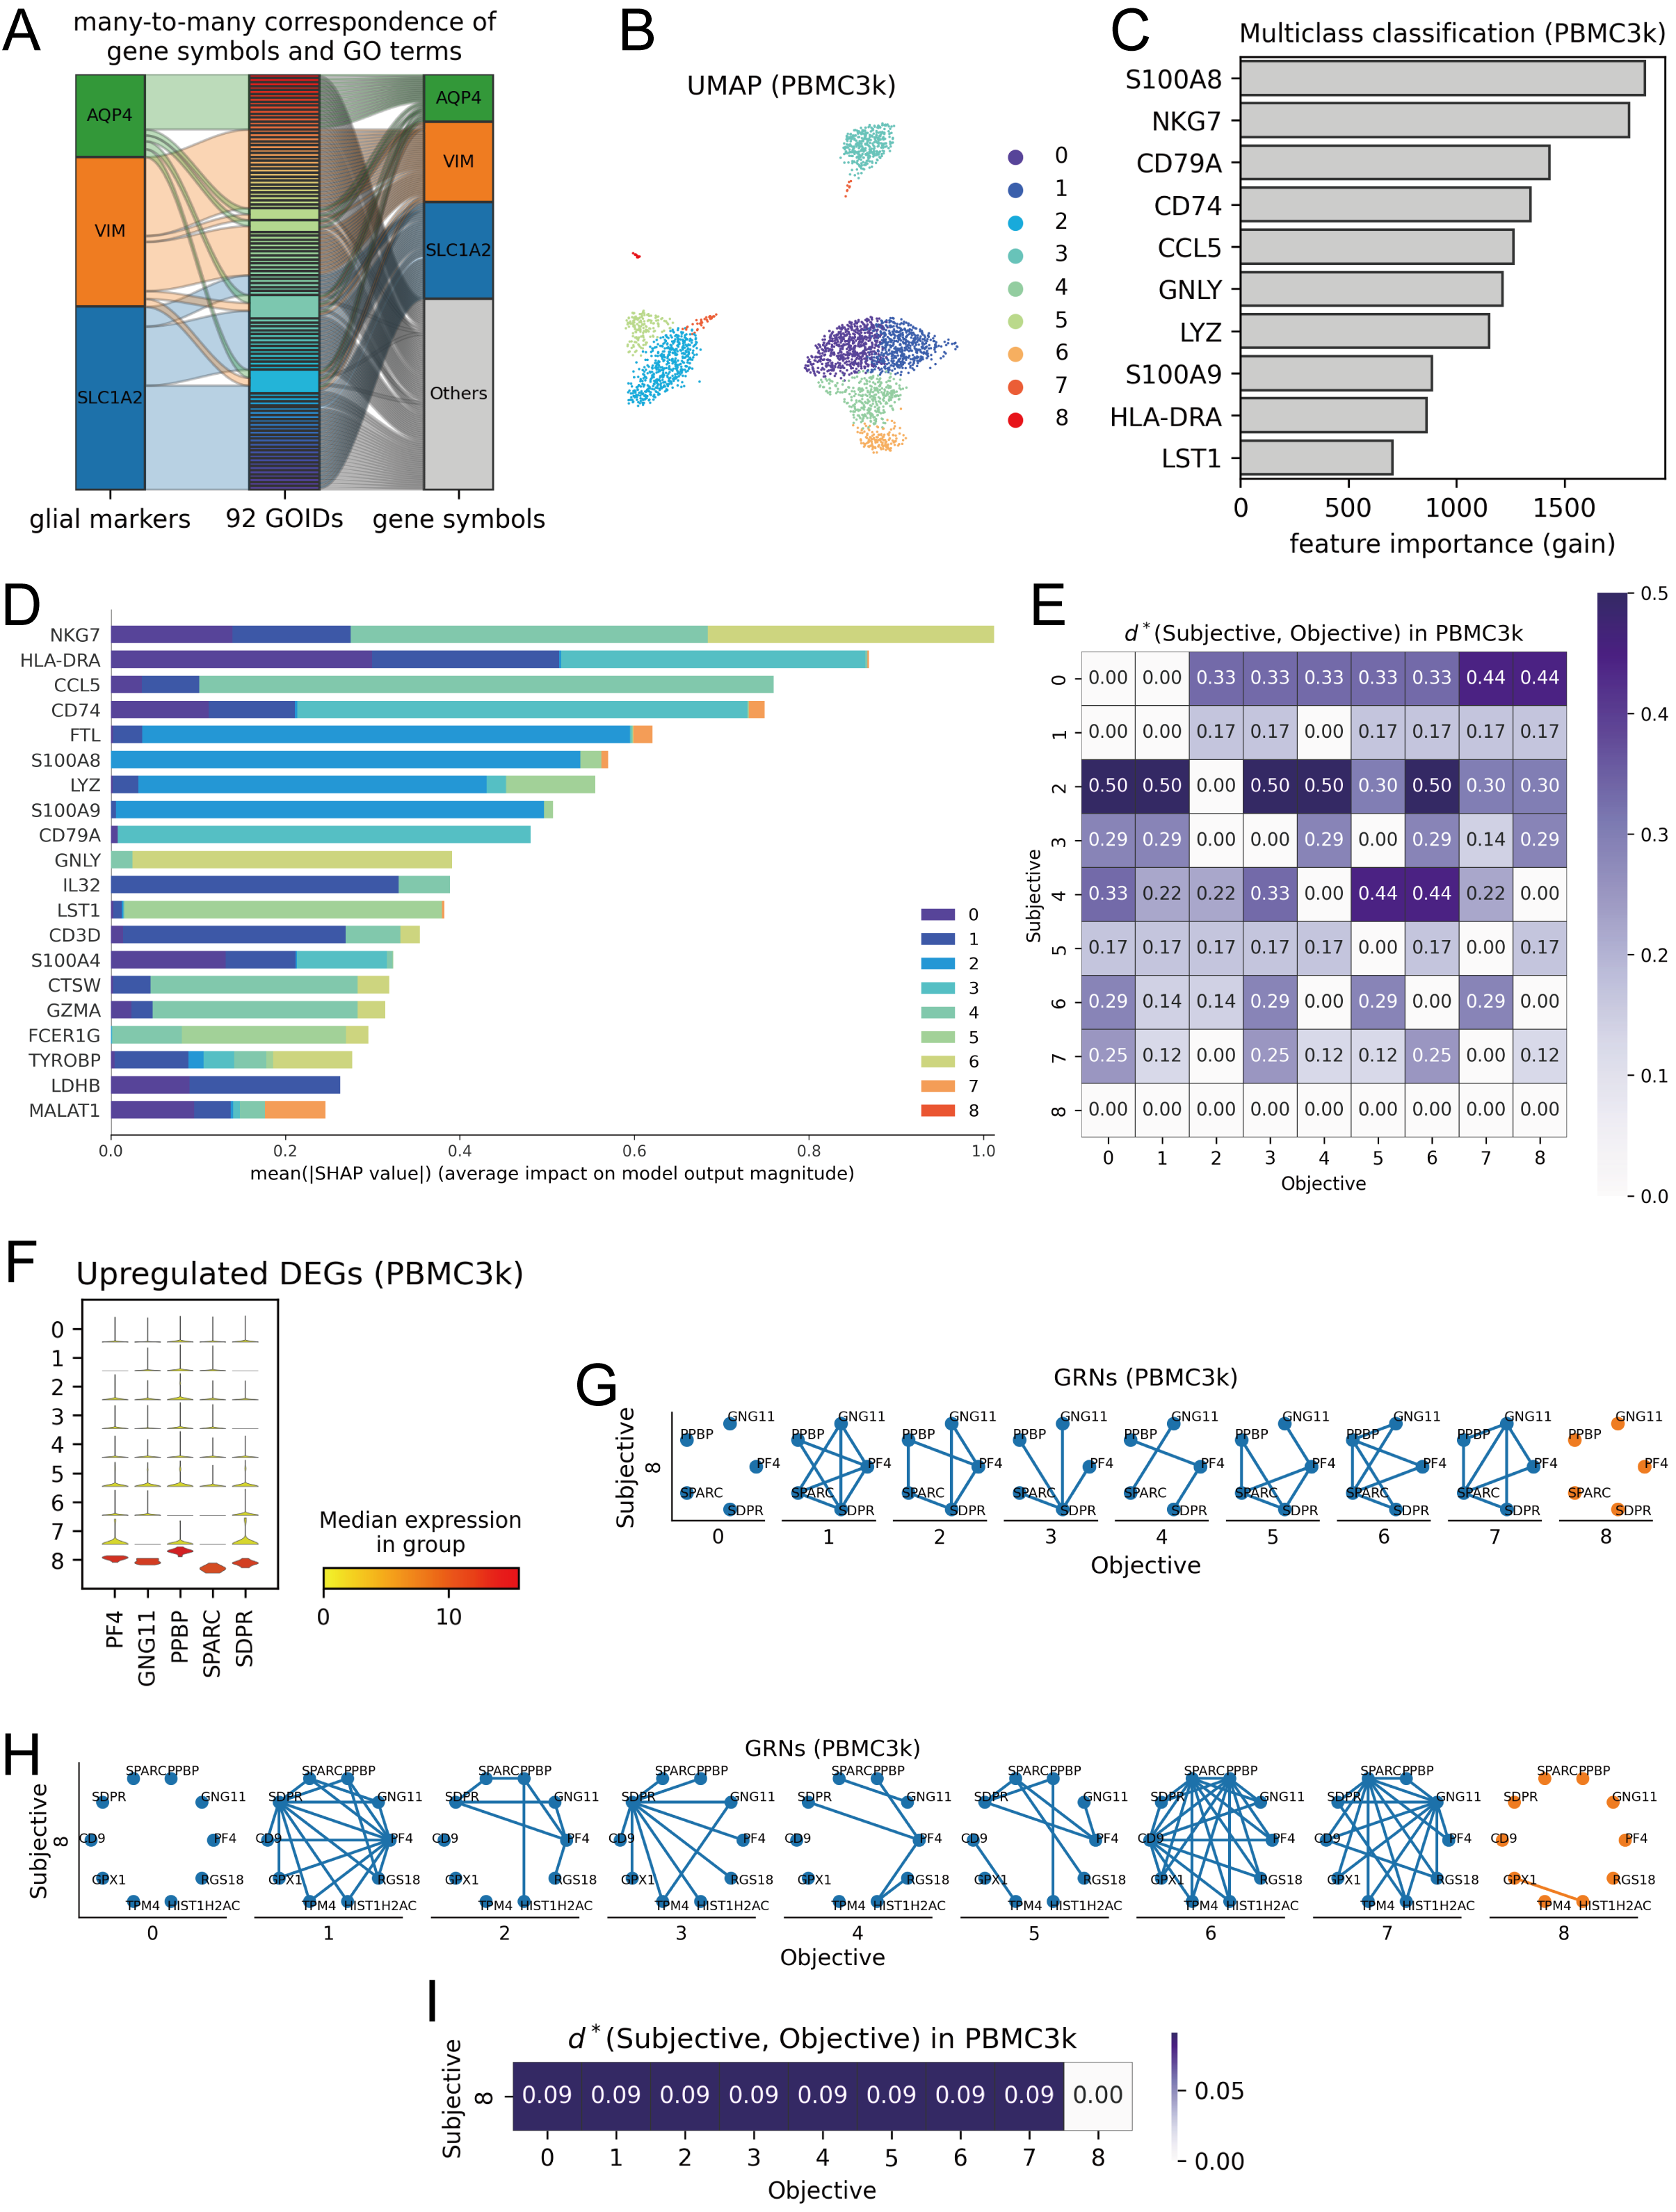
\includegraphics[scale=0.7]{./figs/exported/figure_2.png}
  \caption{Examples of the major issues on the GRN-based frameworks}
  \label{bc}
  \legend{
    \textbf{A}: Alluvial plot showing the many-to-many correspondence between gene symbols and GO terms.
    \textbf{B}: UMAP of the PBMC3k dataset. The markers are colored according to the cluster.
    \textbf{C}: The top 10 genes with the highest feature importance according to the multiclass classification LightGBM model.
    \textbf{D}: The top 20 genes with the highest mean SHAP values according to the multiclass classification LightGBM model.
    \textbf{E}: The $d^*$ values based on the GRNs of the top 5 DEGs. 
    The rows correspond to the subjective cell classes, and the columns correspond to the objective ones.
    \textbf{F}: The top 5 DEGs of cluster 8.
    \textbf{G}: The GRNs of the clusters 0$\sim$8 based on the top 5 DEGs of cluster 8.
    \textbf{H}: The GRNs of the clusters 0$\sim$8 based on the top 10 DEGs of cluster 8.
    \textbf{I}: The re-calculated $d^*$ values among the GRNs based on the top 10 DEGs of cluster 8.
  }
\end{figure}


\subsection*{Semi-automated marker-gene suggestion}
Manual curation of marker genes for GRNs struggles with arbitrariness and incompleteness, while semi-automated 
ML-based and DEG-based methods often require overly recurrsive trials to find optimal sets of marker genes. To 
improve workflow efficiency, we developed an algorithm to automatically suggest similar genes to supplement given 
marker genes. 

We leveraged overlapping GO terms of the given marker genes and mapped them back to gene symbols. For 
instance, the three glial marker genes in our example share two GO terms in their intersection (\figurename{ 3A}), and the 
similarities of their GO terms can be set-theoretically defined with Jaccard index values (\figurename{ 3B}). We interpreted 
that: 1) the intersection of the Venn diagram contained the pivotal GO terms that reflected the biological semantics 
collectively defined by the given marker genes; and 2) the minimal Jaccard index value was the indicator of the 
similarity about the group of genes (therefore it could work as a threshold of acceptance when other genes are 
added). To find new genes without altering the biological meaning of the list, we querried gene symbols tagged 
with the pivotal GO terms (\figurename{ 3C}), filtered out genes that exhibited lower Jaccard index values compared to 
any gene in the original list (\figurename{ 3D}), and used the remainders to form the new gene list (\figurename{ 3E}).

We also implemented a combined method of manual and ML-based marker gene selection on the GRN-based 
annotation using a referential dataset. This labeling evaluates the $d^*$ values from the referential clusters to the query 
clusters. Such methods that require manual assignment of marker genes are suitable for characterizing clusters of 
known cellular identities (i.e., pre-annotated clusters in referential datasets). Accordingly, our new proposal can be 
applied to similar cases.


\begin{figure}[htb]
  \centering
  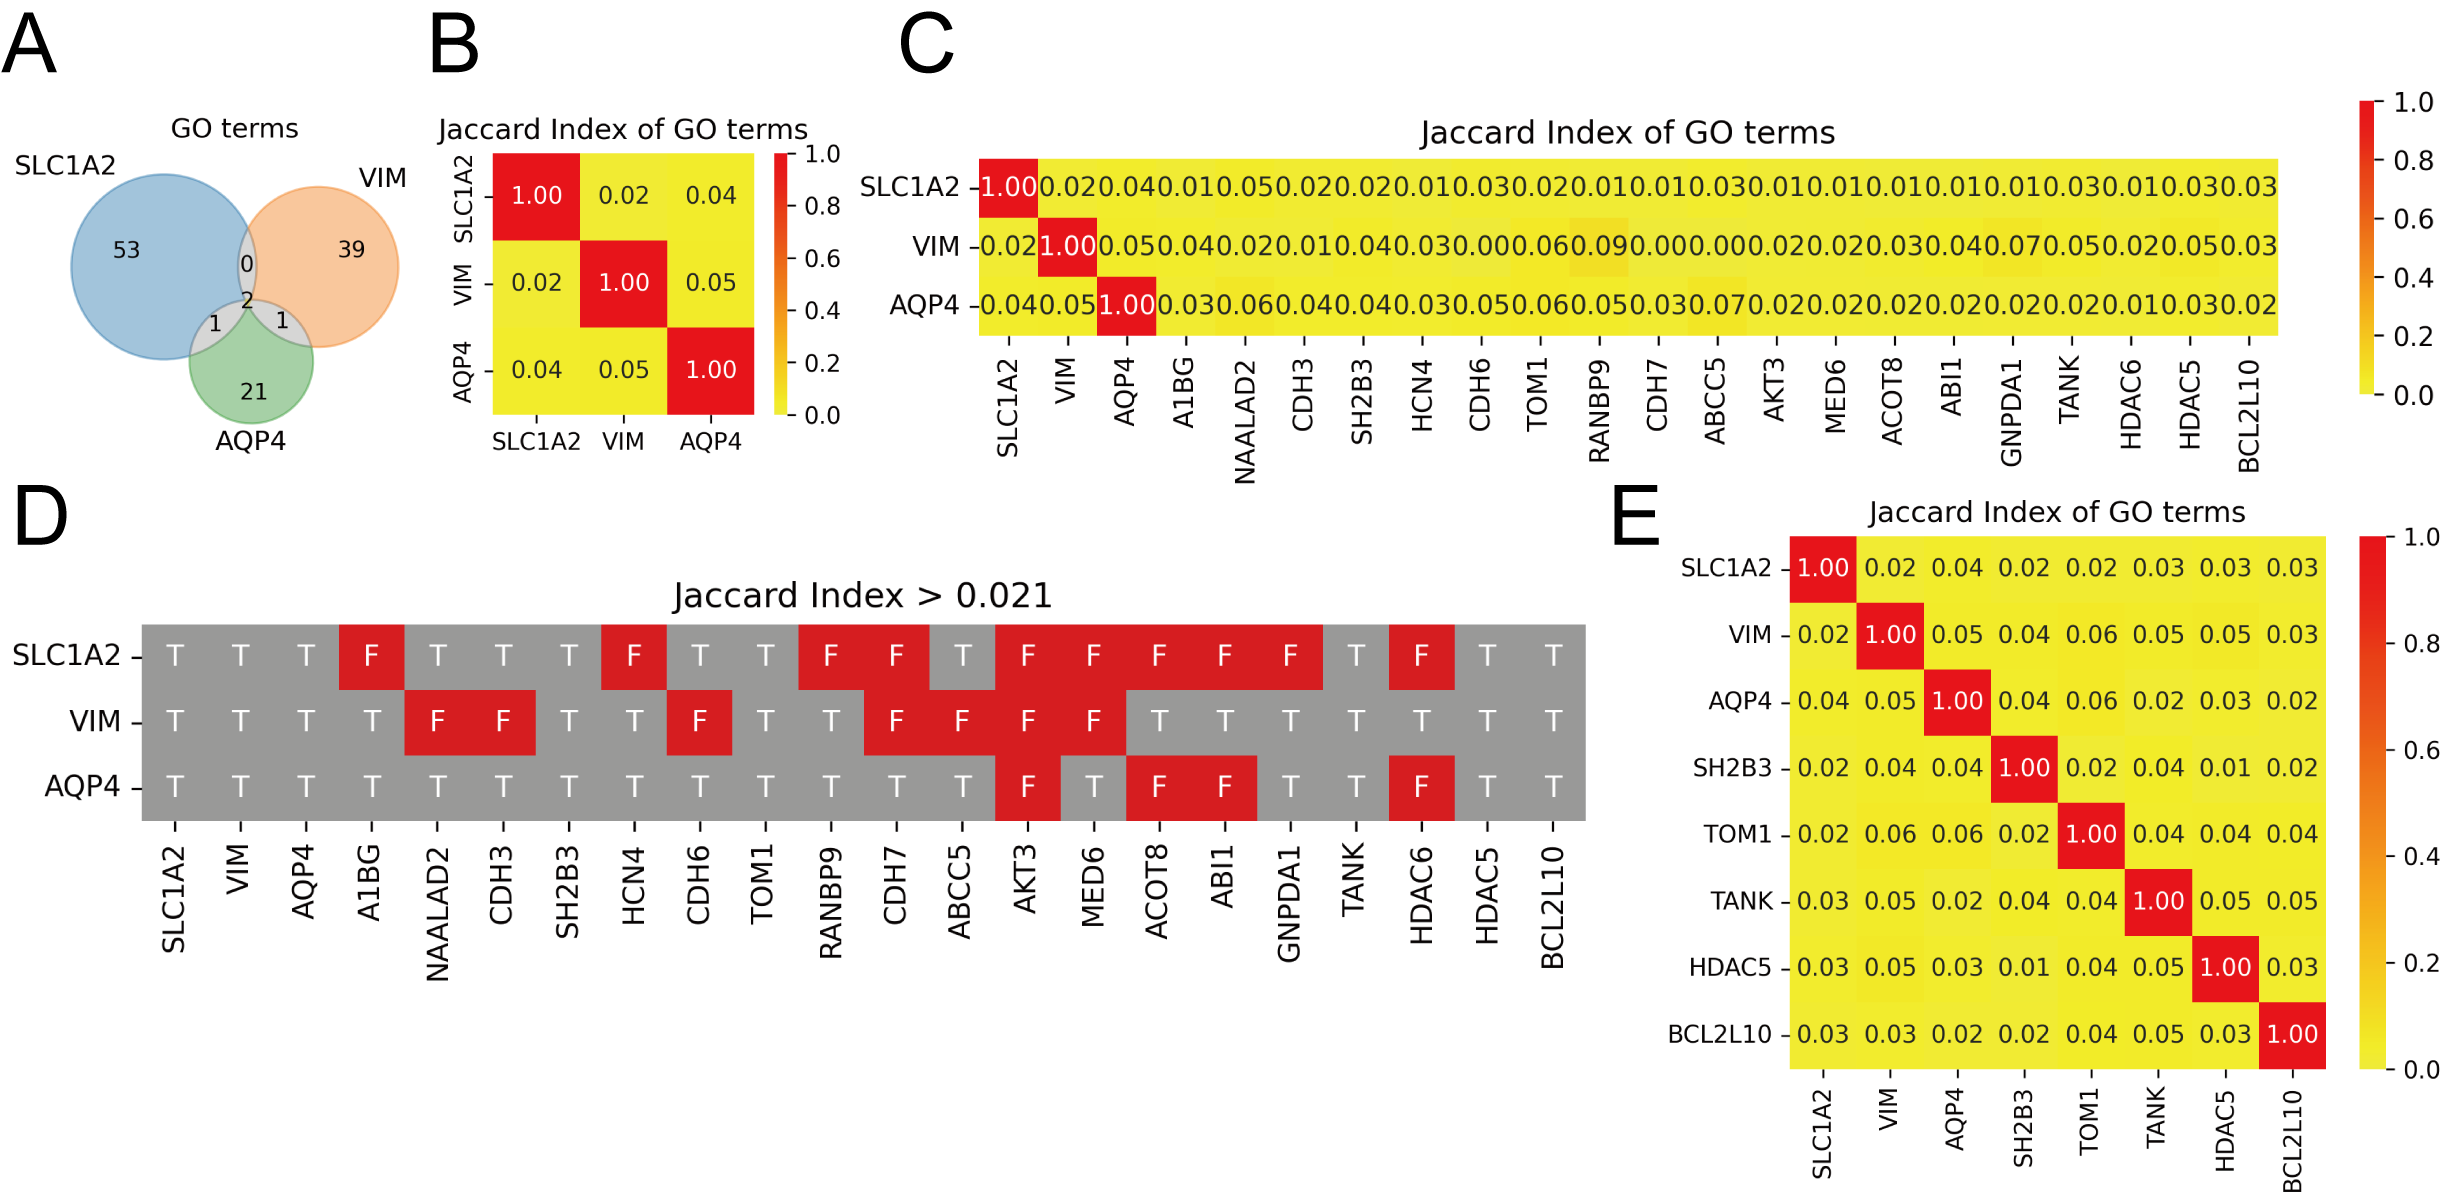
\includegraphics[scale=0.7]{./figs/exported/figure_3.png}
  \caption{Jaccard index based automated marker gene suggestion}
  \label{jibased}
  \legend{
    \textbf{A}: Venn diagram of the GO terms related to the three glial marker genes. 
    Here, we considered the intersection of the three sets as the pivotal GO terms defined by the three marker genes.
    \textbf{B}: Jaccard index values of the GO terms related to the three glial marker genes.
    The minimal value was adopted as the threshold for automated gene selection.
    \textbf{C}: Jaccard index values of the GO terms related to the three glial marker genes and 
    other gene symbols subscribed to the pivotal GO terms.
    \textbf{D}: Jaccard index values smaller than the threshold are shown in red, and the others are shown in gray.
    \textbf{E}: Jaccard index values of the GO terms related to the gene symbols included in the output gene list.
  }
\end{figure}


\subsection*{Dropout-based binarization}
As discussed, the risk of dropout highlights the pitfalls of the correlation-based algorithms. However, recent studies 
show that the zero inflation is closely related to data attributes like cell types \cite{qiu2020embracing, zappia2017splatter}. Building on this, we consider 
dropouts as potential indicators of enriched gene expressions. Our binarization algorithm marks non-zero expression 
values as positive and zeros as negative. For instance, the top two DEGs of cluster 8 in PBMC3k, \textit{PF4} and \textit{GNG11} 
(both megakaryocyte markers \cite{puhm2023diversity}), were rarely expressed in cluster 5 (\figurename{ 2F}). Consequently, the 
$2\times 2$ contingency table identified the majority of cluster 5 as double-negative (\figurename{ 4A}).

While we consider dropout a practically useful feature, some experts oppose this and have developed dropout 
imputation algorithms \cite{kim2020demystifying}. To clarify our point, we here examine how dropouts explain the data features.

First, we validated whether the \ac{DOR}---the proportion of zeros in the count data of a gene---was 
associated with the mean values ($log_2(RPM+1)$) in the PBMC3k data. Although the DOR values and the mean values 
exhibited a non-linear correspondence, we could successfully establish a linear formulation with a simple logistic 
transformation on the mean expression values (See Appendices for details). The logistic-transformed mean values 
fitted well to the linear calibration curve, achieving a coefficient of determination ($R^2$) of 0.993. Additionally, 
the inverse-transformed curve aligned well with the data distribution in the scatter plot of the mean values and the 
DOR (\figurename{ 4B}). Hence, we could demonstrate that the DOR values are closely related to the mean expression values, 
which are the most frequently used summary statistics. As the DOR values are comparable across different 
datasets, while the mean expression values are unsuitable for trans-dataset comparison, it was suggested that the potential 
of the calibration curve of DOR and the mean expression could work effectively in cell class comparison using multiple 
data sources by interchangeably translating the comparable feature and the non-comparable but 
meaningful one. To benchmark the performance of the model, we coined the name ``\ac{LM}'', and 
compared it with a Poisson regression model and a \ac{NB} regression model (\figurename{ 4C}), which 
are well-known models for explaining dropout events \cite{choi2020bayesian}. The \ac{MSE} scores of those models 
indicated that the LM best fitted to the PBMC3k dataset compared to the other competitors (\figurename{ 4D}), and 
its \ac{MAE} (i.e., expected prediction error) in DOR value turned out to be less than 0.005 
(\figurename{ 4E}). To measure the errors produced when turning DOR values back to mean expressions, we made inverse 
prediction models of those three models (See Appendices for details) and tested their performance. As described in 
Appendices, all inverse prediction models have a fundamental issue in predicting mean expression values for zero 
DOR, so we excluded those data from performance evaluation. We visualized \ac{MaxAE} 
values in addition to MAE values to quantify the prediction performance for data of low DOR. LM exhibited the 
lowest MAE, scoring less than 0.1 errors in mean expression values on average (\figurename{ 4F}), and it performed 
the best in MaxAE as well (\figurename{ 4G}).

\begin{figure}[htb]
  \centering
  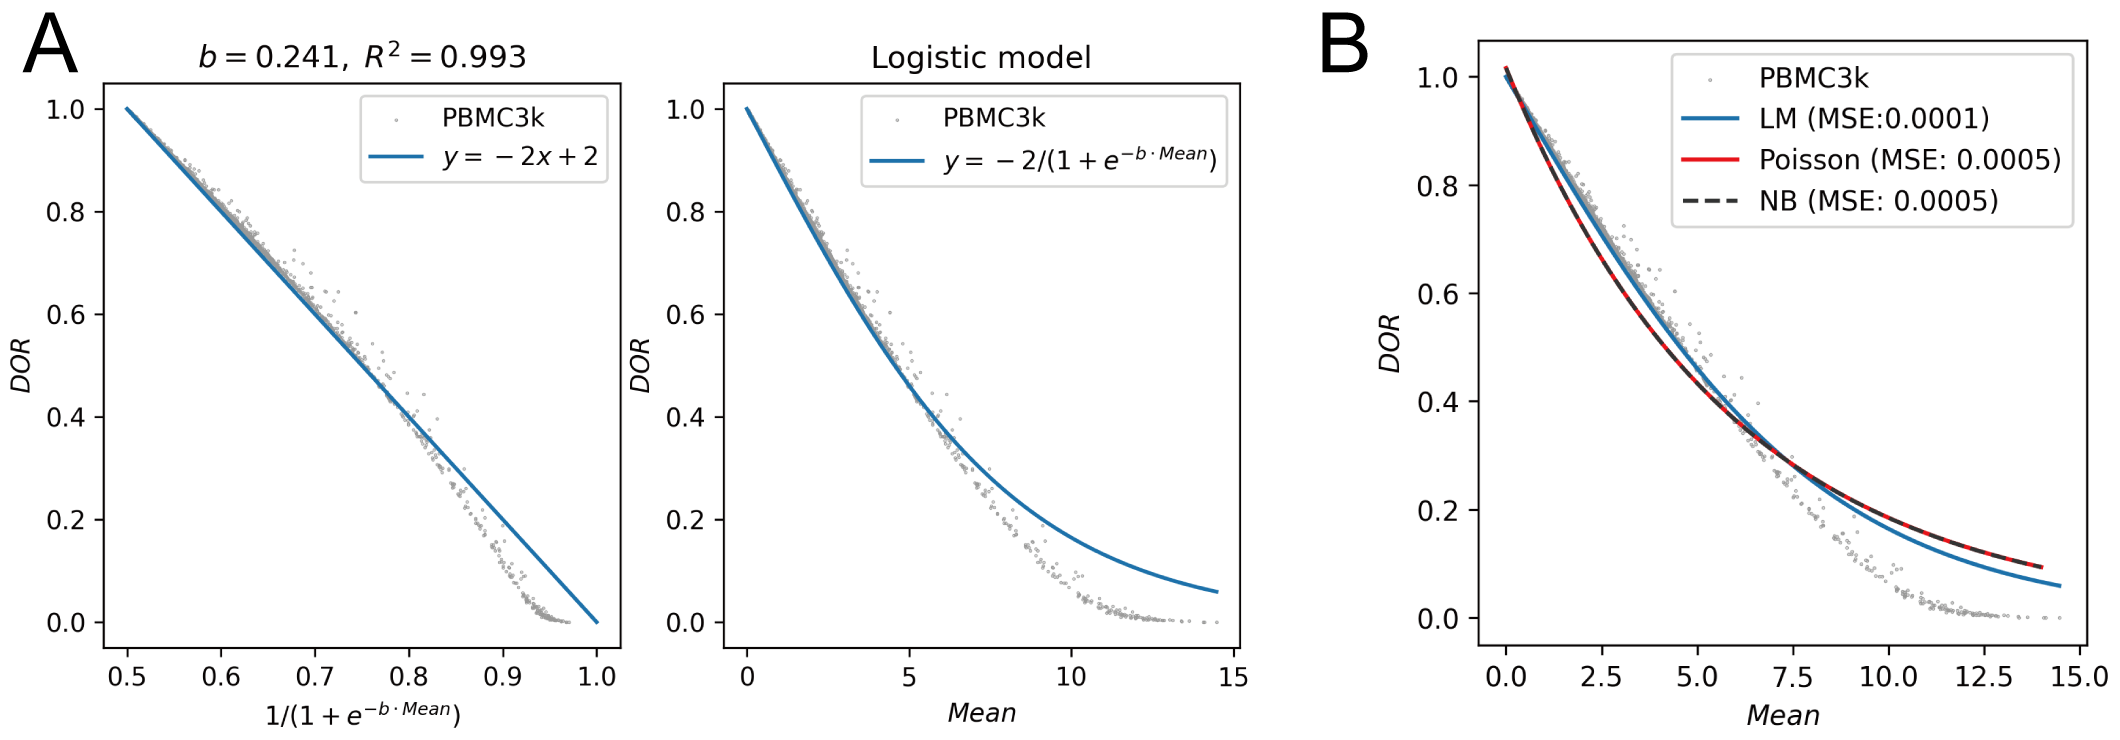
\includegraphics[scale=0.8]{./figs/exported/logisticmodel.png}
  \caption{Dropout-based binarization and empirical investigations on DOR}
  \legend{
    \textbf{A}: A dropout-based $2\times 2$ contingency table of \textit{PF4} and \textit{GNG11} for cluster 5 in PBMC3k 
    ($+$, non-zero expression values; $-$, zeros).
    \textbf{B}: The LM of DOR. 
    \textbf{C}: The performance comparison with the Poisson regression model (Poisson) and 
    the negative-binomial regression model (NB).
    \textbf{D}: Performance comparison of LM, Poisson, and NB with MSE values.
    \textbf{E}: Performance comparison of LM, Poisson, and NB with MAE values.
    \textbf{F}: Performance comparison of the inverse predictions of LM, Poisson, and NB with MAE values.
    \textbf{G}: Performance comparison of the inverse predictions of LM, Poisson, and NB with MaxAE values.
  }
  \label{logistic model}
\end{figure}

Following this, we tested if there is correspondence between DOR and some data attributes unique to individual 
datasets using a group of datasets that we have named ``Mereu2020'' as they were obtained in 2020 by Mereu 
and colleagues \cite{mereu2020benchmarking}. Mereu2020 includes 15 superfamilies where the same sample components were measured across 
different protocols (e.g., different platforms or different sequencing depths) in order to benchmark scRNA-seq 
protocols \cite{mereu2020benchmarking}, including Chromium V2 (deep), Chromium V2 (shallow), Chromium V2 (sn), Chromium V3, C1HT-medium, 
C1HT-small, CEL-seq2, Drop-seq, ICELL8, MARS-Seq, Quartz-Seq2, gmcSCRB-seq, ddSEQ, inDrop, 
and Smart-Seq2; for detailed descriptions, please refer to the original article \cite{mereu2020benchmarking} and URLs of the corresponding 
webpages on Gene Expression Omnibus that we provide in Methods. Datasets included in Mereu2020 exhibit a 
wide range of variations in sample sizes and total reads (\figurename{ S6A}). When we visualized the coverages of gene 
expressions (in other words, proportions of non-zero values which are equivalent to $1-DOR$), numbers of \ac{UMI}, 
and total reads per sample, the datasets with high coverages were found enriched in UMI and read counts (\figurename{ S6B-D}). Thus, DOR appears to reflected those metadata attributes, as was discussed in previous studies \cite{qiu2020embracing, zappia2017splatter}. Furthermore, we tested whether we could accurately reproduce LMs explaining the intertwinement 
between DOR and mean expressions when using Mereu2020 datasets (\figurename{ S7A-O}). As we showed with the 
PBMC3k dataset, logistic-transformed mean expression values of all Mereu2020 datasets fitted well to the linear 
calibration curves, with high coefficients of determination (\figurename{ S8A}). We also benchmarked LMs by 
comparing them with Poisson and NB regression models using those datasets (\figurename{ S7A-O, S8B-E}). As detailed 
in Appendices, the LM demonstrated its capability to function as a calibration curve for DOR and mean expression values 
across a wide range of datasets. Thus, our analysis indicates that DOR reflects metadata features and per-gene characteristics. 
Based on the provided examples, we concluded that DOR can be a useful statistic reflecting 
collective features of scRNA-seq data, including mean expression values and metadata such as sequencing depth 
information.

\subsection*{Weighted evaluation function}
As stated above, the GRN formation dismisses actual mean expression values of a cell cluster by encoding only 
the co-occurrence (or co-absence) of gene expressions. To address this issue, we introduced a new metric that can 
serve as an evaluation function of GRNs instead of $d^*$. This allows us to assign weights to the similarity of graph 
structures based on the abundance of gene expressions. To quantify gene expression amounts comparably across 
different datasets, we used coverage (the presence of non-zero gene expressions, equivalent to $1-DOR$), expecting 
DOR to indirectly reflect the mean expressions of the marker genes forming the edges of the GRNs. With a map 
$q: \Gamma\times X\rightarrow \mathbb{N}$ that returns raw gene counts for gene $\forall g\in\Gamma$ for sample $\forall x\in X$ (where $\Gamma$ is the whole set of genes 
and $X$ is the whole set of samples), we formulated the coverage function $Coverage_{[x]}: \Gamma\rightarrow\mathbb{Q}$ of cell class $[x]$ 
(indicating the coverage value of the given gene $g$ in the designated cell class $[x]$) as follows:
\begin{equation}\label{coverage}
  Coverage_{[x]}(g):=\frac{
    |\{x\;|\;x\in[x]\;s.t.\;q(g,x)\neq 0\}|
  }{
    |[x]|
  }.
\end{equation}
Note that $Coverage_{[x]}$ relies on $q$ only for identifying zeros in raw counts; therefore, any kind of values converted 
from raw counts by a transformation $\psi: \mathbb{N}\rightarrow\mathbb{R}$ such that $\psi^{-1}[\{0\}]=\{0\}$ can be used instead of $q(g, x)$. For 
instance, \ac{RPM} values and $\log_2(RPM+1)$ are accepted (see Appendices for more detailed explanations).

Given that Eq.\eqref{d_asterisk} can also be denoted as Eq.\eqref{HQPM}, we introduced our new evaluation function, the \ac{WHQPM} 
$Whqpm$, by multiplying the cardinality of the gene set $|G|$ respectively 
with the coverage values resulting in Eq.\eqref{WHQPM}:

\begin{equation}\label{HQPM}
  d^*([x], [y]) := 1 - \frac{|C_{[x]}(G)\cap C_{[y]}(G)|}{|C_{[x]}(G)|}
  =1 - \frac{
    |E_{[x]}(G)\cap E_{[y]}(G)|+|G|
  }{
    |E_{[x]}(G)|+|G|
  }
\end{equation}
\begin{equation}\label{WHQPM}
  Whqpm([x], [y]) := 1 - \frac{
    |E_{[x]}(G)\cap E_{[y]}(G)|+\sum_{g\in G}Coverage_{[y]}(g)
  }{
    |E_{[x]}(G)|+\sum_{g\in G}Coverage_{[x]}(g)
  }.
\end{equation}
Note that \ac{WHQPM} cannot be defined if $Coverage_{[x]}(g)=0$ for all $\forall g\in G$, and this property of WHQPM prohibits 
a cell class from being assigned similarity to other cell classes based on totally irrelevant genes exhibiting zero 
expressions (See also Appendices for detailed explanations).

As WHQPM depends on coverage values, not only biological variations but also technical factors including 
choices of sequencing pipelines affect the result. If one considers that differences in DOR are also realistic features 
of the data, WHQPM is available for comparing cell classes across different datasets. Otherwise, \ac{OT}-based 
domain adaptation can mitigate the gap if the experimenter prefers to standardize the various effects 
that impact on DOR, as described in \figurename{ S9A-H} and Appendices.

To demonstrate the benefit of using WHQPM, we first computed GRNs of the clusters 0 through 8 on their top 5 DEGs using the dropout-based binarization technique and the PC algorithm for categorical data (\figurename{ 5A}), 
and then calculated $Whqpm$ values to visualize the similarities of the clusters (\figurename{ 5B}). Although the PC algorithm for categorical data inferred the exact same GRNs for different clusters in some cases (e.g., the GRNs of 
the top 5 DEGs of cluster 8, namely \textit{PF4}, \textit{GNG11}, \textit{PPBP}, \textit{SPARC}, and \textit{SDPR}), $Whqpm$ distinguished the differences 
between cluster 8 and the other clusters as it returned non-zero values except for cluster 8 itself. As $d^*$ returns zero 
if the subjective cell class has no edges in its GRN, we could resolve this issue with WHQPM.


\begin{figure}[htb]
  \centering
  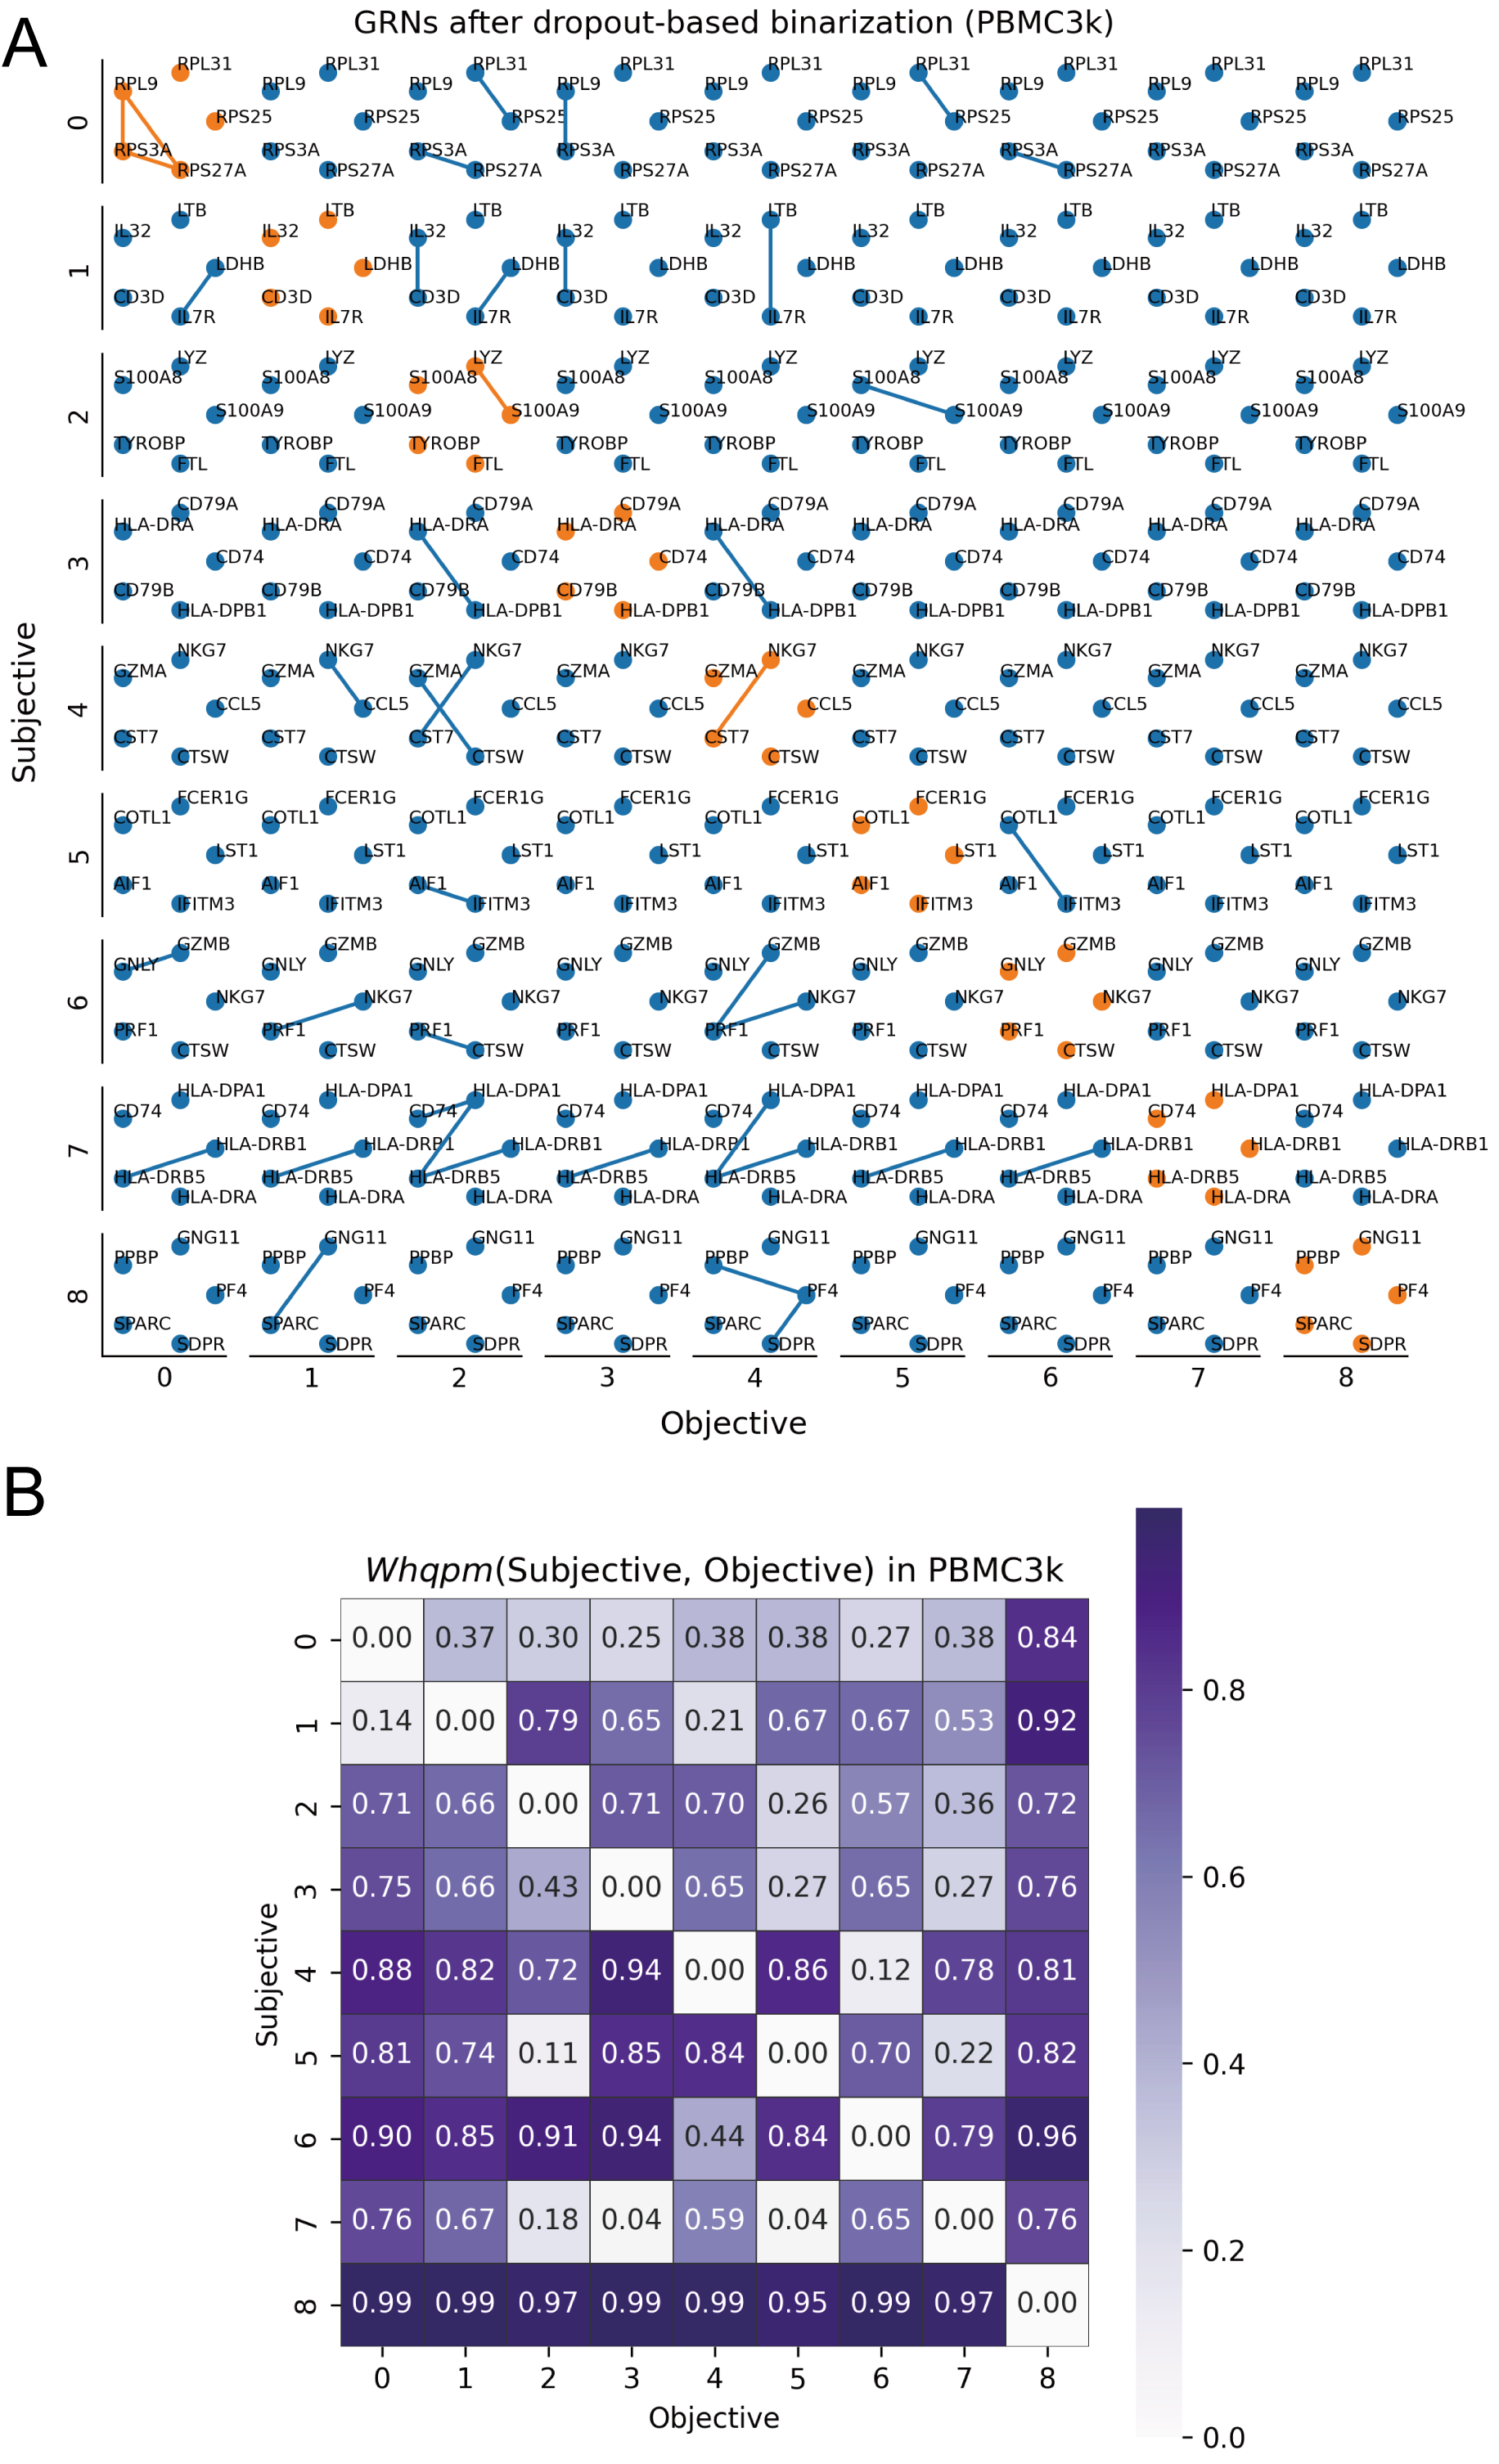
\includegraphics[scale=0.8]{./figs/exported/binarization.png}
  \caption{Combination of dropout-based binarization and WHQPM}
  \legend{
    \textbf{A}: GRNs of the clusters in PBMC3k generated with dropout-based binarization and the PC algorithm for categorical data. 
    GRNs in a row share the same set of genes (DEGs of the subjective clusters) selected for the vertex sets.
    \textbf{B}: The $Whqpm$ values based on the GRNs of the top 5 DEGs generated after dropout-based binarization.
  }
  \label{binarization}
\end{figure}


\section*{Discussion}
In general, scRNA-seq data processing is driven by statistical, geometrical, and information-theoretical approaches, 
even though the results from these algorithms are validated by their ability to recite the storyline of biology. In 
other words, the specific details of algorithms are not necessarily interesting as long as the results make biological sense. Therefore, 
heuristics is often valued over theoretical rigor. As scRNA-seq data accumulate at an accelerating rate, 
and despite their sensitivity to fluctuations in surrounding conditions, we believe that a framework that can handle 
scRNA-seq data in a tentative but comparable format will help balance context-dependency and generalization, 
uncovering universal truth yet to be unveiled.

We previously designed the GRN-based definition of cellular identities and the metric $d^*$ to quantify their 
similarity levels. However, our method included several impracticalities, as described earlier in this article. Therefore, 
we proposed a series of solutions aimed at improving functionality. Additionally, we launched a Python package, 
GRNet (pronounced garnet), to provide a platform for our proposed concepts. While promising results have been 
observed in a limited number of datasets, broader validation and discussion is still required.

\section*{Methods}
\subsection*{GRNet Implementations}

\subsubsection*{GO term-assisted gene selection using Jaccard Index}
The Jaccard Index of two sets $A, B$ is defined as:
\begin{equation}\label{jaccard}
  J(A, B) := \frac{A\cap B}{A\cup B}.
\end{equation}
We expanded this definition to pairwise comparisons of multiple elements by forming a matrix where each element is 
the corresponding Jaccard Index. We named this matrix the \ac{JIM}. As an example, the 
element in the $i$-th row and $j$-th column (where $i, j, k\in\mathbb{N}$ and $i\leq k, j\leq k$) is defined as follows when a JIM of 
sets $X_1, X_2,\cdots, X_k$ is introduced:
\begin{equation}\label{jim}
  JIM_{i, j} := J(X_i, X_j).
\end{equation}

When a collection of genes $g_1, \cdots, g_k$ collectively explain a certain type of cells, and they are tagged with respective 
sets of GO terms $G_1, \cdots, G_k$, we considered $min_{i,j\in\{1\cdots k\}}J(G_i, G_j)$ as a threshold of biological correspondence 
to the type of cells. For example, let $G_{k+1}, G_{k+2}$ be the sets of GO terms tagged with $g_{k+1}$ and $g_{k+2}$ 
($g_{k+1}, g_{k+2}\notin \{g_1, \cdots, g_k\}$); then a new gene $g_{k+1}$ would be important for the type of cells if $min_{i\in\{1\cdots k\}}J(G_i, G_{k+1})$ 
is less than $min_{i,j\in\{1\cdots k\}}J(G_i, G_j)$, and $g_{k+2}$ would be irresponsible if $min_{i\in\{1\cdots k\}}J(G_i, G_{k+2})$ is greater than 
$min_{i,j\in\{1\cdots k\}}J(G_i, G_j)$. Under those rules, we implemented a search for important markers from genes tagged with 
GO terms in $\bigcap_{i\in\{1,\cdots,k\}}G_i$.

For detailed implementation, we calculated the JIM of the related GO terms of given seed markers. We used 
mygene.py \cite{mygene} to query the GO database, and Numpy \cite{numpy} to calculate JIM.

\subsubsection*{GRNs and the evaluation function}
Following our previous report \cite{okano2023set}, we implemented a correlation-baed PC algorithm for GRN formation and the evaluation 
function $d^*$ for similarity of GRN structures using Numpy, Pandas \cite{pandas}, and pgmpy. Additionally, we 
implemented dropout-based binarization, a chi-squared test-based PC algorithm, and WHQPM accordingly.


\subsection*{scRNA-seq data analysis}
\subsubsection*{Dataset List}
The scRNA-seq data we used in this research were publicly available from the following online resources:

\begin{itemize}
  \item PBMC3k: \url{https://support.10xgenomics.com/single-cell-gene-expression/datasets/1.1.0/pbmc3k}
  \item Mereu2020: \url{https://www.ncbi.nlm.nih.gov/geo/query/acc.cgi?acc=GSE133549}
  \begin{itemize}
    \item Chromium V2 (deep): \url{https://www.ncbi.nlm.nih.gov/geo/query/acc.cgi?acc=GSE133535}
    \item Chromium V2 (shallow): \url{https://www.ncbi.nlm.nih.gov/geo/query/acc.cgi?acc=GSE133536}
    \item Chromium V2 (sn): \url{https://www.ncbi.nlm.nih.gov/geo/query/acc.cgi?acc=GSE133546}
    \item Chromium V3: \url{https://www.ncbi.nlm.nih.gov/geo/query/acc.cgi?acc=GSE141469}
    \item C1HT-medium: \url{https://www.ncbi.nlm.nih.gov/geo/query/acc.cgi?acc=GSE133537}
    \item C1HT-small: \url{https://www.ncbi.nlm.nih.gov/geo/query/acc.cgi?acc=GSE133538}
    \item CEL-seq2: \url{https://www.ncbi.nlm.nih.gov/geo/query/acc.cgi?acc=GSE133539}
    \item Drop-seq: \url{https://www.ncbi.nlm.nih.gov/geo/query/acc.cgi?acc=GSE133540}
    \item ICELL8: \url{https://www.ncbi.nlm.nih.gov/geo/query/acc.cgi?acc=GSE133541}
    \item MARS-Seq: \url{https://www.ncbi.nlm.nih.gov/geo/query/acc.cgi?acc=GSE133542}
    \item Quartz-Seq2: \url{https://www.ncbi.nlm.nih.gov/geo/query/acc.cgi?acc=GSE133543}
    \item gmcSCRB-seq: \url{https://www.ncbi.nlm.nih.gov/geo/query/acc.cgi?acc=GSE133544}
    \item ddSEQ: \url{https://www.ncbi.nlm.nih.gov/geo/query/acc.cgi?acc=GSE133547}
    \item inDrop: \url{https://www.ncbi.nlm.nih.gov/geo/query/acc.cgi?acc=GSE133548}
    \item Smart-Seq2: \url{https://www.ncbi.nlm.nih.gov/geo/query/acc.cgi?acc=GSE133545}
  \end{itemize}
\end{itemize}

\subsubsection*{Preprocessing, dimensionality reduction, and visualization}
We performed data preprocessing, dimensionality reduction, and data visualization of the scRNA-seq datasets 
using Python packages (including Scanpy \cite{scanpy}, Polars \cite{polars}, Pandas, Numpy, Matplotlib \cite{matplotlib}, and Seaborn \cite{seaborn}).

\subsubsection*{Clustering and DEA}
We performed leiden clustering, and \ac{DEA} using Scanpy.

\subsubsection*{Multiclass classification GBDT model}
We randomly split the PBMC3k data into training, validation, and test data (3:1:1). Using the training and 
validation data, we created a GBDT model minimizing the multiclass-logarithmic loss function using LightGBM's 
framework \cite{lightgbm}. We implemented the model with a wrapper in Optuna \cite{optuna} to automatically tune the hyperparameters. 
The models performance was tested with ROC curves and PR curves using Scikit-learn \cite{scikit-learn} and Matplotlib. 
We also visualized the feature importance values implemented in LightGBM. SHAP scores were calculated and 
visualized with the Shap Python package \cite{shap,shap_treeexplainer}.

\subsubsection*{GO analysis}
We performed the GO analysis using gprofiler2 \cite{gprofiler2}, and visualized the results with Matplotlib and Seaborn.

\subsubsection*{Statistical models of DOR and the benchmarking}
For LM, we optimized $b$ of the calibration curve by minimizing the MSE between $DOR$ and $\frac{2}{1+e^{-b\cdot Mean}}+2$ with 
AdaGrad. We implemented LM and plotting functions with AnnData, Matplotlib, Numpy, Pandas, and PyTorch \cite{pytorch}. 
We implemented Poisson regression models with Statsmodels \cite{statsmodels}. For NB regression models, we built them 
on Statsmodels and optimized hyperparameters using Optuna.

\subsubsection*{OT-based coverage standardization}
We made OT-based domain adaptation models using the EMDTransport class of POT \cite{pot} with the squared 
Euclidean cost. The results were visualized with Matplotlib, Numpy, Pandas, and Seaborn.

\subsection*{Other visualizations}
\subsubsection*{Alluvial plot and Venn diagram for GO terms}
The glial markers were selected based on review articles, and the tagged GO terms were queried using mygene.py. 
Then, all gene symbols subscribed with each GO terms were queried again. The alluvial plot was created with 
Matplotlib, Numpy, and Pandas, and the Venn diagram was visualized with Matplotlib-Venn \cite{matplotlib-venn}.

\section*{Code availability}
GRNet and the analysis codes are available on GitHub at \url{https://github.com/yo-aka-gene/grnet}. Online documentation 
for GRNet is also provided at \url{https://grnet.readthedocs.io}.


\section*{Author contributions}
\begin{description}
  \item[Conceptualization] YO
  \item[Methodology] YO
  \item[Implementation] YO
  \item[Investigation] YO
  \item[Visualization] YO
  \item[Funding acquisition] YO, YK, HO
  \item[Project administration] YO, YK, HO
  \item[Supervision] HO
  \item[Senior author] YK
  \item[Original draft] YO
  \item[Editing] YK, HO
\end{description}

\section*{Acknowledgements}
This work was supported by the Keio University Medical Science Fund (to YO). We are grateful to Dr. Hans 
Dijkstra (Fujita Health University) for critical reading of the manuscript.


\section*{Abbreviations}
\printacronyms[heading=Abbreviations]

\bibliographystyle{ieeetr}
\bibliography{refs.bib}
\end{document}
